\SourcePage{664}{669}
\section{High-energy asymptotic behavior of scattering amplitudes}

We shall examine the asymptotic behavior, at high energies, of the amplitudes and cross sections for two-particle scattering processes $(1+2\to3+4)$. For the principal electrodynamic processes, the answer in the first nonvanishing order in $\alpha$ can be obtained from the explicit formulas derived in the preceding chapters, which hold at arbitrary energies. Here we instead approach the question more generally, so that these asymptotic forms can be found directly.

As in \S~66, introduce the invariant variables
\begin{equation}
s=(p_1+p_2)^2,\qquad t=(p_1-p_3)^2,\qquad u=(p_1-p_4)^2
\tag{134.1}
\end{equation}
(with $p_1+p_2=p_3+p_4$); this notation refers to reactions in the $s$-channel, which are the ones considered below. In the ultrarelativistic case, when the energies greatly exceed the particle masses, the two particle energies in the center-of-mass frame are approximately equal. If $\varepsilon$ denotes the sum of the colliding-particle energies, then in this frame $p_1=(\varepsilon/2,\,\mathbf p_1)$, $p_2=(\varepsilon/2,\,-\mathbf p_1)$, $p_3=(\varepsilon/2,\,\mathbf p_3)$, $p_4=(\varepsilon/2,\,-\mathbf p_3)$, $\mathbf p_1^2=\mathbf p_3^2=\varepsilon^2/4$, and hence
\begin{equation}
s=\varepsilon^2,\qquad t=-\frac{s}{2}(1-\cos\theta),\qquad
u=-\frac{s}{2}(1+\cos\theta),
\tag{134.2}
\end{equation}
where $\theta$ is the angle between $\mathbf p_1$ and $\mathbf p_2$.

First consider the asymptotic form of the reaction cross section at a fixed value of the scattering angle $\theta$. All three variables $s$, $t$, and $u$ are then proportional to one another and tend to infinity simultaneously. Particle masses cannot enter the result in the ultrarelativistic case, and the only quantity having the dimension of length is $1/\varepsilon$ ($=\hbar c/\varepsilon$). Dimensional considerations alone therefore show that the differential cross section for a two-particle reaction decreases with energy according to the asymptotic law
\begin{equation}
d\sigma/do\propto1/s\qquad\text{for}\qquad s,\ |t|,\ |u|\to\infty.
\tag{134.3}
\end{equation}
If the cross section is referred to the differential $dt$ rather than to the solid-angle element $do$, then, since $do\propto dt/s$,
\begin{equation}
d\sigma/dt\propto1/s^2.
\tag{134.4}
\end{equation}
In the ultrarelativistic case the cross section is related to the scattering amplitude by $d\sigma/dt\propto|M_{fi}|^2/s$; see (64.22),(64.23). Thus (134.3) means that in the asymptotic limit the scattering amplitude has no dependence on $s$:
\begin{equation}
M_{fi}=\mathrm{const}.
\tag{134.5}
\end{equation}

\SourcePage{665}{670}
As is evident from the nature of the argument, these results apply not only in the first nonvanishing approximation, but also in higher orders of perturbation theory (that is, with radiative corrections included), provided logarithmic factors such as $\ln(s/m^2)$ are disregarded. Dependence on dimensionless logarithms plainly cannot be determined by dimensional reasoning\footnote{Summing series that contain logarithmic corrections can produce an exponential dependence on the logarithms, thereby changing the exponent in the power law. This change is small, however, because $\alpha$ is small.}.

The situation differs when $s$ is increased at fixed $t$, that is, at a fixed squared momentum transfer. In other words, one considers scattering through small angles that diminish as the energy rises:
\begin{equation}
s\to\infty,\qquad |t|\sim s\theta^2=\mathrm{const},\qquad
\theta\sim(|t|/s)^{1/2}.
\tag{134.6}
\end{equation}
In this case dimensional analysis tells us only that the total power of $1/s$ and $1/t$ in $d\sigma/dt$ is 2 (and that in the amplitude $M_{fi}$ it is zero)\footnote{Here the fixed value of $|t|$ is assumed to satisfy $|t|\gg m^2$. The results obtained in this way remain valid as regards their dependence on $s$ (that is, on the energy) also when $|t|\sim m^2$.}. To find the part of the cross section that decreases most slowly with increasing $s$, one must therefore isolate the factor with the highest power of $1/t$. Such factors arise only when a Feynman diagram can be divided into two parts, separating the ends $1$, $3$ from $2$, $4$, by cutting virtual-particle lines. The total four-momentum carried by these lines is $p_1-p_3$, which is the origin of the factor's dependence on $t=(p_1-p_3)^2$. Thus the asymptotic form of a diagram in the region (134.6) is governed by the possible cuts of the diagram in the $t$-channel.

Similarly, the asymptotic behavior in the region
\begin{equation}
s\to\infty,\qquad |u|\sim s(\pi-\theta)^2=\mathrm{const},\qquad
|\pi-\theta|\sim(|u|/s)^{1/2},
\tag{134.7}
\end{equation}
which corresponds to scattering through angles near $\pi$, is determined by the possible cuts of the diagram in the $u$-channel (that is, between the ends $1$, $4$ and $2$, $3$).

The simplest example is electron--electron scattering, represented by the diagrams (73.13) and (73.14). Of these, the first admits a $t$-channel cut through the virtual-photon line; it consequently determines the asymptotic behavior of the scattering amplitude in the region (134.6). The $D$-function associated with the virtual-photon line is proportional to $1/t$. The asymptotic forms of the am\SourcePageJoin{666}{671}plitude and differential scattering cross section are therefore
\begin{equation}
M_{fi}\propto s/t,\qquad d\sigma\propto dt/t^2.
\tag{134.8}
\end{equation}
The asymptotic behavior in the limit (134.7), near the backward direction, is instead fixed by the ``exchange'' diagram (73.14); in this limit
\[
M_{fi}\propto s/u,\qquad d\sigma\propto du/u^2.
\]
For mutual scattering of unlike particles (an electron and a muon), there is no exchange diagram. Its cross section for scattering through angles $\theta\approx\pi$ therefore decreases according to (134.3),(134.4)\footnote{These statements are, of course, consistent with the results of \S~81; see (81.11) and problem~6.}.

We shall show that including radiative corrections does not alter these results for the asymptotic behavior of electron--electron scattering. To do so, consider corrections of different kinds to diagram (73.13).

We have already seen that diagrams representing corrections to the internal $D$-function (see (113.11)) or to the vertex parts (see (117.1)) produce only logarithmic corrections to the amplitude; they do not change the power dependence in (134.8). The same is true of a diagram that can be cut through two internal photon lines instead of one:
\begin{equation}
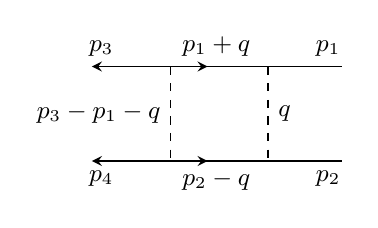
\begin{tikzpicture}[baseline=-.45ex,x=1cm,y=1cm,>=stealth,line width=.6pt,font=\small]
  \coordinate (tl) at (-.62,.72);
  \coordinate (tr) at (.62,.72);
  \coordinate (bl) at (-.62,-.48);
  \coordinate (br) at (.62,-.48);
  \draw[<-] (-1.62,.72)--(1.56,.72);
  \draw[<-] (-1.62,-.48)--(1.56,-.48);
  \draw[dashed] (tl)--(bl);
  \draw[dashed] (tr)--(br);
  \draw[<-] (-.15,.72)--(-.16,.72);
  \draw[<-] (-.15,-.48)--(-.16,-.48);
  \node[above] at (-1.50,.72) {$p_3$};
  \node[above] at (1.38,.72) {$p_1$};
  \node[below] at (-1.50,-.48) {$p_4$};
  \node[below] at (1.38,-.48) {$p_2$};
  \node[above] at (-.04,.72) {$p_1+q$};
  \node[below] at (-.04,-.48) {$p_2-q$};
  \node[left] at (-.62,.12) {$p_3-p_1-q$};
  \node[right] at (.62,.12) {$q$};
\end{tikzpicture}
\tag{134.9}
\end{equation}
The scattering amplitude belonging to this diagram differs from that of diagram (73.13) by replacing the factor $1/t$ with
\[
\frac{\bigl(\gamma(p_1+q)\bigr)\bigl(\gamma(p_2-q)\bigr)}
{(p_1+q)^2(p_2-q)^2q^2(p_3-p_1-q)^2}\,d^4q
\]
and then integrating over $d^4q$. The relevant integration region is the one that yields the smallest power of $1/s$. For this purpose $q$ must in any event be small in comparison with $p_1$ and $p_2$. Dropping terms that are small in this sense, as well as the terms $p_1^2=p_2^2=m^2$, we may rewrite this expression as
\begin{equation}
\frac{(\gamma p_1)(\gamma p_2)}{(p_1q)(p_2q)q^2(p_3-p_1-q)^2}\,d^4q.
\tag{134.10}
\end{equation}

\SourcePage{667}{672}
The denominator contains no $s$ if $q_0$ and $q_x$ (the $x$ axis lies along $\mathbf p_1=-\mathbf p_2$) are proportional to $1/\sqrt{s}$, while the components $q_y$ and $q_z$ may be proportional to $1/\sqrt{|t|}$; the integration region is then proportional to $1/s$. The numerator, on the other hand, is of order $p_1p_2\propto s$. Consequently, replacing one internal photon line in the diagram by two does not change its dependence on $s$ at fixed $t$\footnote{We emphasize once more that only power-law asymptotics are at issue, so logarithmic divergences in the integration may be disregarded. Diagrams of the type (134.9) will be studied in greater detail in \S~137.}. In other words, the contribution of diagram (134.9) to the scattering amplitude obeys the same asymptotic law (134.8) as the basic diagram. The conclusion remains unchanged if further parallel internal photon lines are added to the diagram, or if corrections to the internal electron lines are inserted.

This result is general: every diagram that can be divided into two parts in the $t$-channel or the $u$-channel by cutting any number of internal photon lines contributes to the amplitude with the respective asymptotic behavior $M_{fi}\propto s/t$ for $t=\mathrm{const}$ or $s/u$ for $u=\mathrm{const}$ (\emph{V.~G.~Gorshkov, V.~N.~Gribov, L.~N.~Lipatov, G.~V.~Frolov}, 1967; \emph{H.~Cheng, T.~T.~Wu}, 1969).

As another example, consider Compton scattering, which is represented by the two diagrams (74.14). These diagrams admit no cut in the $t$-channel, but the second can be cut in the $u$-channel through the internal electron line; in the notation of this section it is
\begin{equation}
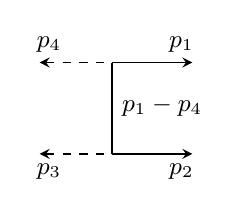
\begin{tikzpicture}[baseline=-.45ex,x=1cm,y=1cm,>=stealth,line width=.6pt,font=\small]
  \coordinate (a) at (0,.58);
  \coordinate (b) at (0,-.58);
  \draw[dashed,<-] (-.92,.58)--(a);
  \draw[<-] (1.02,.58)--(a);
  \draw (a)--(b);
  \draw[dashed,<-] (-.92,-.58)--(b);
  \draw[<-] (1.02,-.58)--(b);
  \node[above] at (-.80,.58) {$p_4$};
  \node[above] at (.88,.58) {$p_1$};
  \node[below] at (-.80,-.58) {$p_3$};
  \node[below] at (.88,-.58) {$p_2$};
  \node[right] at (0,.02) {$p_1-p_4$};
\end{tikzpicture}
\tag{134.11}
\end{equation}
Thus the scattering is concentrated chiefly near the backward direction, as was already noted at the end of \S~86; see (86.20). To obtain the asymptotic behavior in this region, observe that the factor $G$ associated with the internal line of diagram (134.11) is of order $1/\gamma(p_1-p_4)\propto1/\sqrt{|u|}$. Hence the scattering amplitude is $M_{fi}\propto\alpha(s/|u|)^{1/2}$; the factor $\alpha$ has been included because diagram (134.10) is of second order. It follows that the differential cross section is $d\sigma/du\propto\alpha^2/|u|s$. The integral of this expression over $|u|$ is governed by the region $|u|\ll s$. The resulting total cross section decreases with

\SourcePage{668}{673}
increasing energy as $\sigma\propto\alpha^2/s$ (more precisely, $\sigma\propto(\alpha^2/s)\ln(s/m^2)$); compare (86.20)\footnote{The exact dependence of the cross section on $|u|$ or $|t|$ when either is $\lesssim m^2$ cannot, of course, be determined from the considerations given here. It is understood that the integral over $|u|$ (or over $|t|$) converges at values of order $m^2$. This is indeed the case for all processes except elastic scattering of charged particles.}.

For this process, however, radiative corrections do alter the asymptotic behavior. The change comes from sixth-order diagrams of the form
\begin{equation}
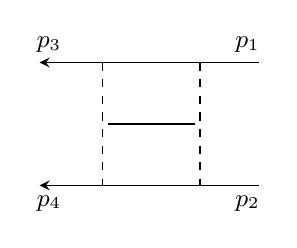
\begin{tikzpicture}[baseline=-.45ex,x=1cm,y=1cm,>=stealth,line width=.6pt,font=\small]
  \coordinate (tl) at (-.62,.78);
  \coordinate (tr) at (.62,.78);
  \coordinate (bl) at (-.62,-.78);
  \coordinate (br) at (.62,-.78);
  \draw[<-] (-1.42,.78)--(1.36,.78);
  \draw[<-] (-1.42,-.78)--(1.36,-.78);
  \draw[dashed] (tl)--(bl);
  \draw[dashed] (tr)--(br);
  \draw (tl)--(tr);
  \draw (-.55,0)--(.55,0);
  \draw (bl)--(br);
  \node[above] at (-1.30,.78) {$p_3$};
  \node[above] at (1.22,.78) {$p_1$};
  \node[below] at (-1.30,-.78) {$p_4$};
  \node[below] at (1.22,-.78) {$p_2$};
\end{tikzpicture}
\tag{134.12}
\end{equation}
They can be cut in the $t$-channel through two internal photon lines and therefore contribute to the amplitude with the asymptotic behavior $M_{fi}\propto\alpha^3s/t$ (the factor $\alpha^3$ corresponds to the diagram's sixth order). At sufficiently large $s$, this part of the amplitude becomes dominant, and the differential cross section is then
\[
d\sigma/dt\propto\alpha^6/t^2.
\]
The integral of this expression over $t$ is governed by the region of small values $|t|\sim m^2$, that is, by scattering angles $\theta\sim m/\sqrt{s}$. Notice that the scattering now takes place chiefly in the forward rather than the backward direction. As a result, the total cross section ceases to decrease with energy:
\begin{equation}
\sigma\propto\alpha^6/m^2=\alpha^4/r_e^2.
\tag{134.13}
\end{equation}
The decreasing part of the cross section becomes comparable with its constant part at $\varepsilon=\sqrt{s}\propto m/\alpha^2$.

An analogous situation occurs in light-by-light scattering. In the first nonvanishing approximation it is represented by the ``box'' diagrams (127.1), which can be cut through two internal electron lines. The four-momentum of these lines is integrated over in the diagram, and the important momenta are of order $\sqrt{s}$; small values of $t$ (or $u$) receive no special emphasis. Hence, for any fixed $t$ (or fixed $u$), the asymptotic behavior of these diagrams is given by (134.5): $M_{fi}=\mathrm{const}\propto\alpha^2$. The total cross section then decreases with increasing energy, $\sigma\propto\alpha^4/s$ (compare (127.23)); angles close to zero or to $\pi$ are not singled out. In eighth order, however, diagrams appear that can be cut in the $t$- or $u$-channel through two

\SourcePage{669}{674}
internal photon lines, for example,
\begin{equation}
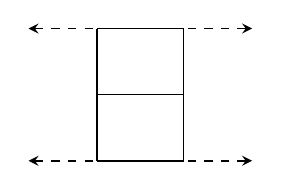
\begin{tikzpicture}[baseline=-.45ex,x=1cm,y=1cm,>=stealth,line width=.6pt]
  \coordinate (tl) at (-.55,.84);
  \coordinate (tr) at (.55,.84);
  \coordinate (bl) at (-.55,-.84);
  \coordinate (br) at (.55,-.84);
  \draw[dashed,<-] (-1.42,.84)--(tl);
  \draw[dashed,<-] (1.42,.84)--(tr);
  \draw[dashed,<-] (-1.42,-.84)--(bl);
  \draw[dashed,<-] (1.42,-.84)--(br);
  \draw (tl)--(bl);
  \draw (tr)--(br);
  \draw (tl)--(tr);
  \draw (-.55,0)--(.55,0);
  \draw (bl)--(br);
\end{tikzpicture}
\tag{134.14}
\end{equation}
These diagrams yield a constant asymptotic cross section: $\sigma\propto\alpha^8/m^2$ when $\sqrt{s}\gg m/\alpha^2$\footnote{The cross section for coherent photon scattering in a nuclear field already has a constant asymptotic form in the first nonvanishing approximation, represented by ``box'' diagrams two of whose ends are external-field lines (see (128.7)). In fact, however, these diagrams ought to be drawn in the form (134.12), with the upper solid line representing the nucleus. The external-field lines then become internal lines of the diagram, and the origin of the constant asymptotic behavior is evident.}.

A constant asymptotic value of the total cross section is characteristic of scattering processes whose diagrams can be cut, in either the $t$- or the $u$-channel, through internal photon lines. The same property also holds when more than two particles are produced in the reaction's final state.
